

\chapter[追踪算法设计]{追踪算法设计}[Harbin Institute of Technology Postgraduate Dissertation Writing Specifications]

\section{引言}[Content specification]
由于画面中可能存在多块装甲板,若要对装甲板建立运动模型必须明确当前装甲板与历史装甲板的
匹配关系,追踪算法的设计目的就在于此。
在目标追踪算法的设计中,高效、准确是核心考虑因素。
尽管基于深度学习的方法在追踪任务中能够获得非常高的准确率,
但其对计算资源的消耗也是不可忽视的。
因此,本文提出了一种算法设计思路,不依赖于深度学习技术。
该算法为每块装甲板单独建立运动模型,利用模型对当前时刻进行位置预测,
并基于类贪心算法
并通过一一配对来实现目标追踪。

\section{追踪算法设计}[Content specification]

算法设计思路为:为每块装甲板单独建立运动模型,每块有运动模型的装甲板利用运动模型对当前时刻进行位置预测,然后与观测到的装甲板进行一一配对,若距离小于阈值且观测装甲板的数字与携带运动模型对应装甲板的数字一致,
则认为两者同属一块装甲板,利用当前装甲板信息更新运动模型,从而实现追踪效果。
为了实现追踪效果的鲁棒性,允许装甲板的运动模型在短时间不更新,从而起到在受遮挡的情况下依然保留运动模型,待装甲板离开遮挡后不必重新计算运动模型;但是较长时间不更新则认为目标已经不在视野范围内。
\par

另外追踪层级有两层,第一级为追踪同一块装甲板,若追踪同一块装甲板失败,则退而求其次,追踪同一辆车。
因为存在识别算法不稳定或者是装甲板被遮挡等因素造成的识别丢帧现象,
所以在追踪模式下(包括追踪同一块装甲板模式和追踪同一辆车模式)允许一定数量的丢帧。
基本思路为:设置三个模式:搜索装甲板模式,追踪装甲板模式,以及追踪车辆模式,
初始状态标记设为搜索装甲板模式。

\begin{itemize}[itemindent=2em]
\item 在搜索装甲板模式下,如果搜索到装甲板则将标记位设置为追踪装甲板模式,且将该装甲板设置为追踪目标。
\item 在搜索装甲板模式下,如果未搜索到装甲板则直接返回。
\item 在追踪装甲板模式下,在装甲板丢帧次数低于追踪通装甲板丢帧阈值的情况下识别到追踪目标,则将装甲板丢帧次数清零,且更新追踪目标为当前检测到的装甲板。
\item 在追踪装甲板模式下,在装甲板丢帧次数低于追踪通装甲板丢帧阈值的情况下未识别到追踪目标,则将次数增加1。
\item 在追踪装甲板模式下,在若装甲板丢帧次数高于追踪通装甲板丢帧阈值的情况下则将标记为设置为追踪车辆模式,且装甲板丢帧次数清零。
\item 在追踪车辆模式下,在车辆丢帧次数低于追踪车辆丢帧阈值的情况下识别到同一辆车的其他装甲板,则将车辆丢帧次数清零,且更新追踪目标为当前检测到的装甲板,且将标记为设置为追踪装甲板模式。
\item 在追踪车辆模式下,在车辆丢帧次数低于追踪车辆丢帧阈值的情况下未识别到同一辆车的其他装甲板,则将车辆丢帧次数加1。
\item 在追踪车辆模式下,在车辆丢帧次数高于追踪车辆丢帧阈值的情况下,将标记为设置为搜索装甲板模式,装甲板丢帧次数清零,车辆丢帧次数清零。
\end{itemize}

追踪逻辑如图\ref{追踪算法逻辑图}所示:

\begin{figure}[H]
    \centering
    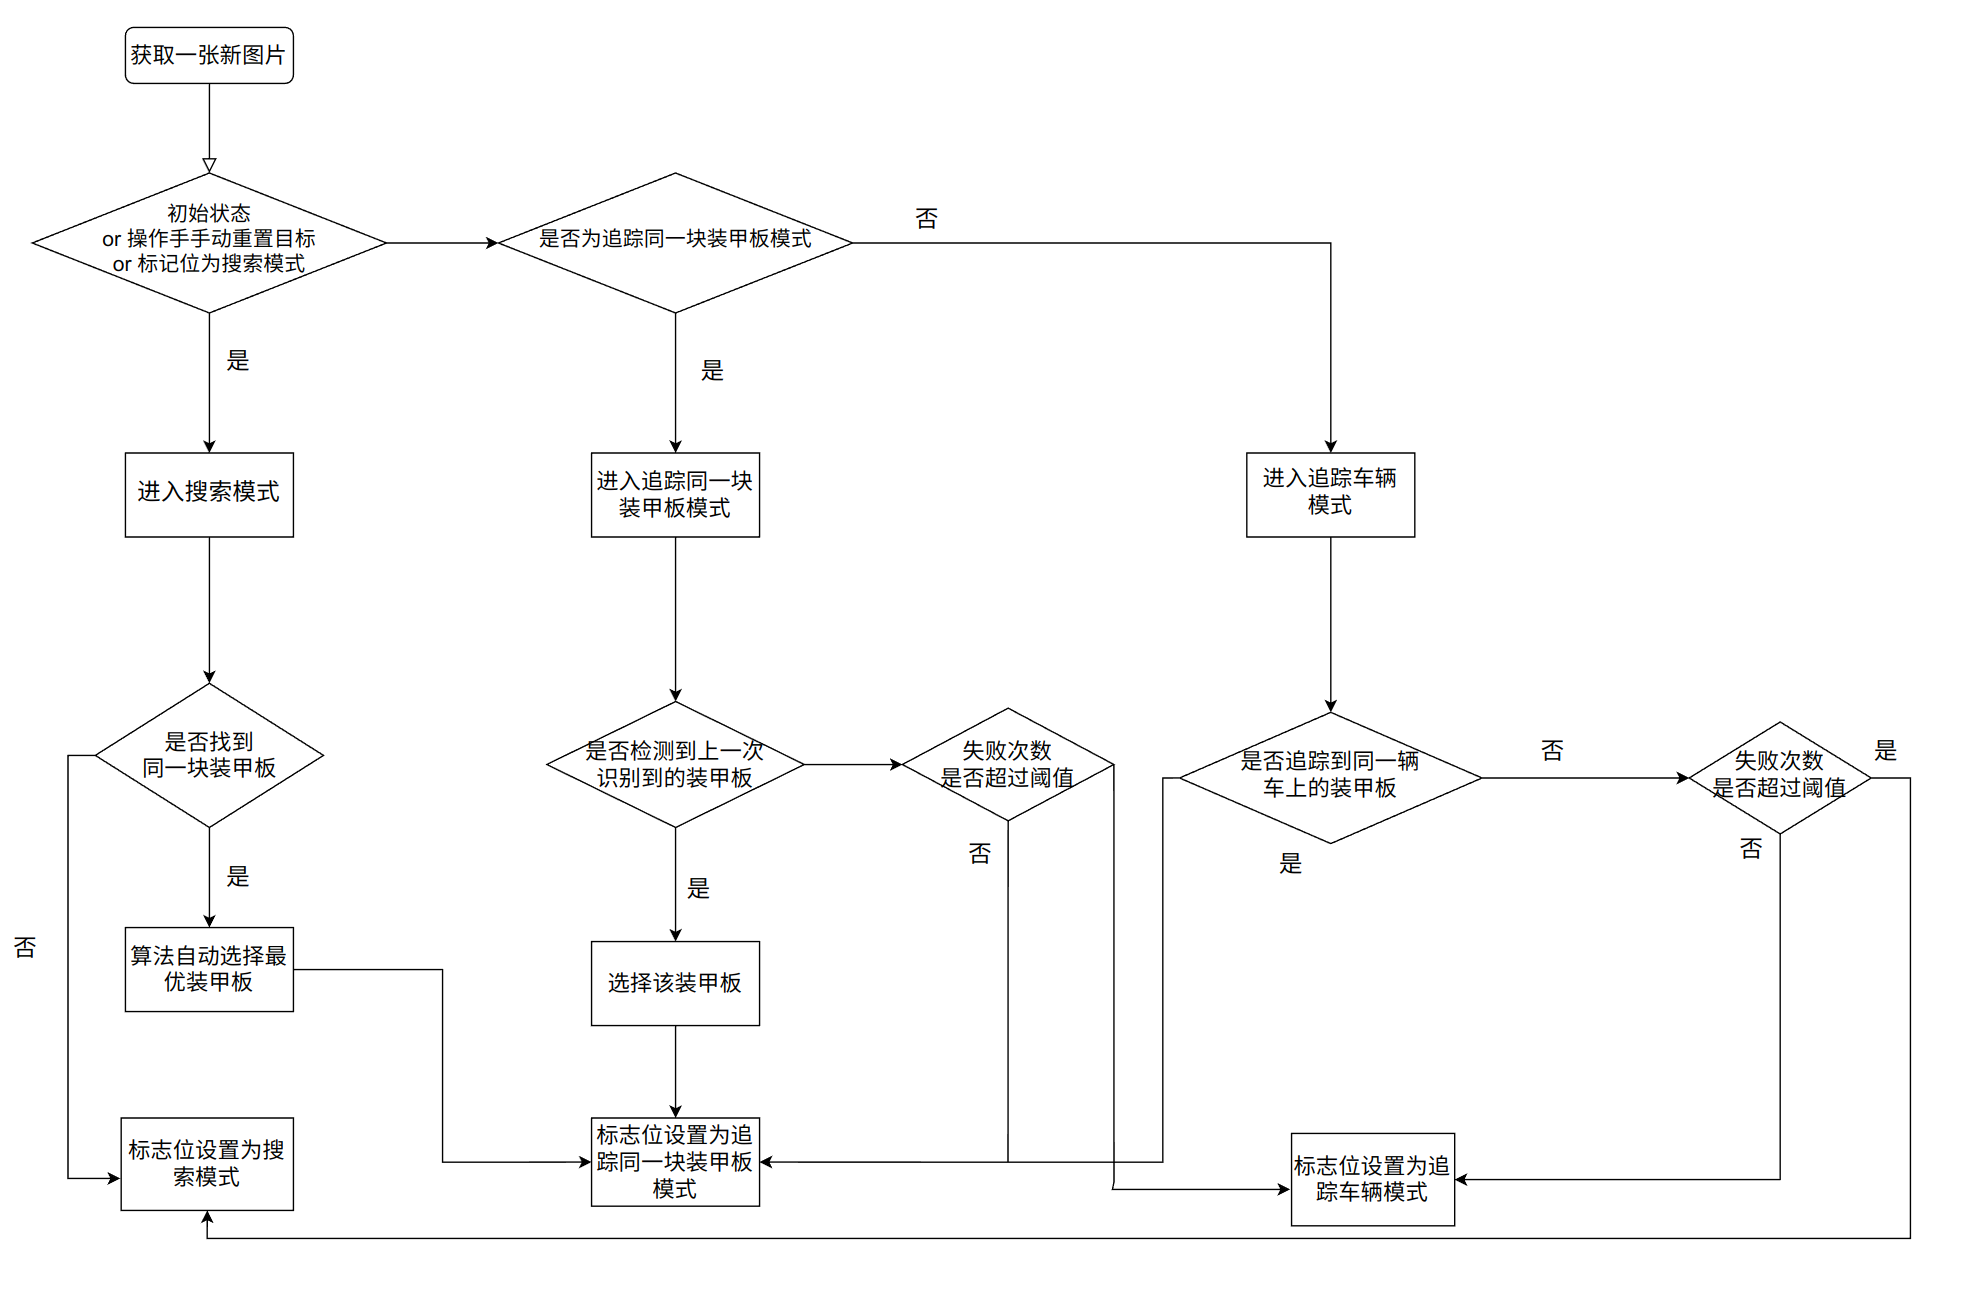
\includegraphics[width=.99\textwidth]{track_chart.png} 
    \caption{追踪算法逻辑图} 
    \label{追踪算法逻辑图} 
\end{figure} 

\par


\section{本章小结}[Content specification]


% 本章基于运动模型的设计了一种追踪算法,目的是为了建立装甲板与历史装甲板之间的匹配关系。
% 该算法为每个装甲板建立单独的运动模型,
% 然后将当前时刻的位置预测与观测到的装甲板进行一一配对,
% 通过更新运动模型来实现追踪效果。该算法设计了两个追踪层级,
% 第一级是追踪同一块装甲板,第二级是退而求其次,追踪同一辆车的不同装甲板。
% 为了提高算法的鲁棒性,该算法允许运动模型在短时间内不更新,
% 从而在装甲板受遮挡时保留运动模型,但长时间不更新则认为目标已不在视野范围内。
% 文章为算法设计了三种模式:搜索装甲板模式、
% 追踪装甲板模式和追踪车辆模式,通过标记位的设置来实现状态的转换。
% 提高算法的鲁棒性。该算法没有使用深度学习方法,注重算法的效率和准确性。
% 实现效果如图\ref{pred_merge}所示,目标从左向右移动,云台也追踪着目标从左向右移动。
% \begin{figure}[H]
%     \centering
%     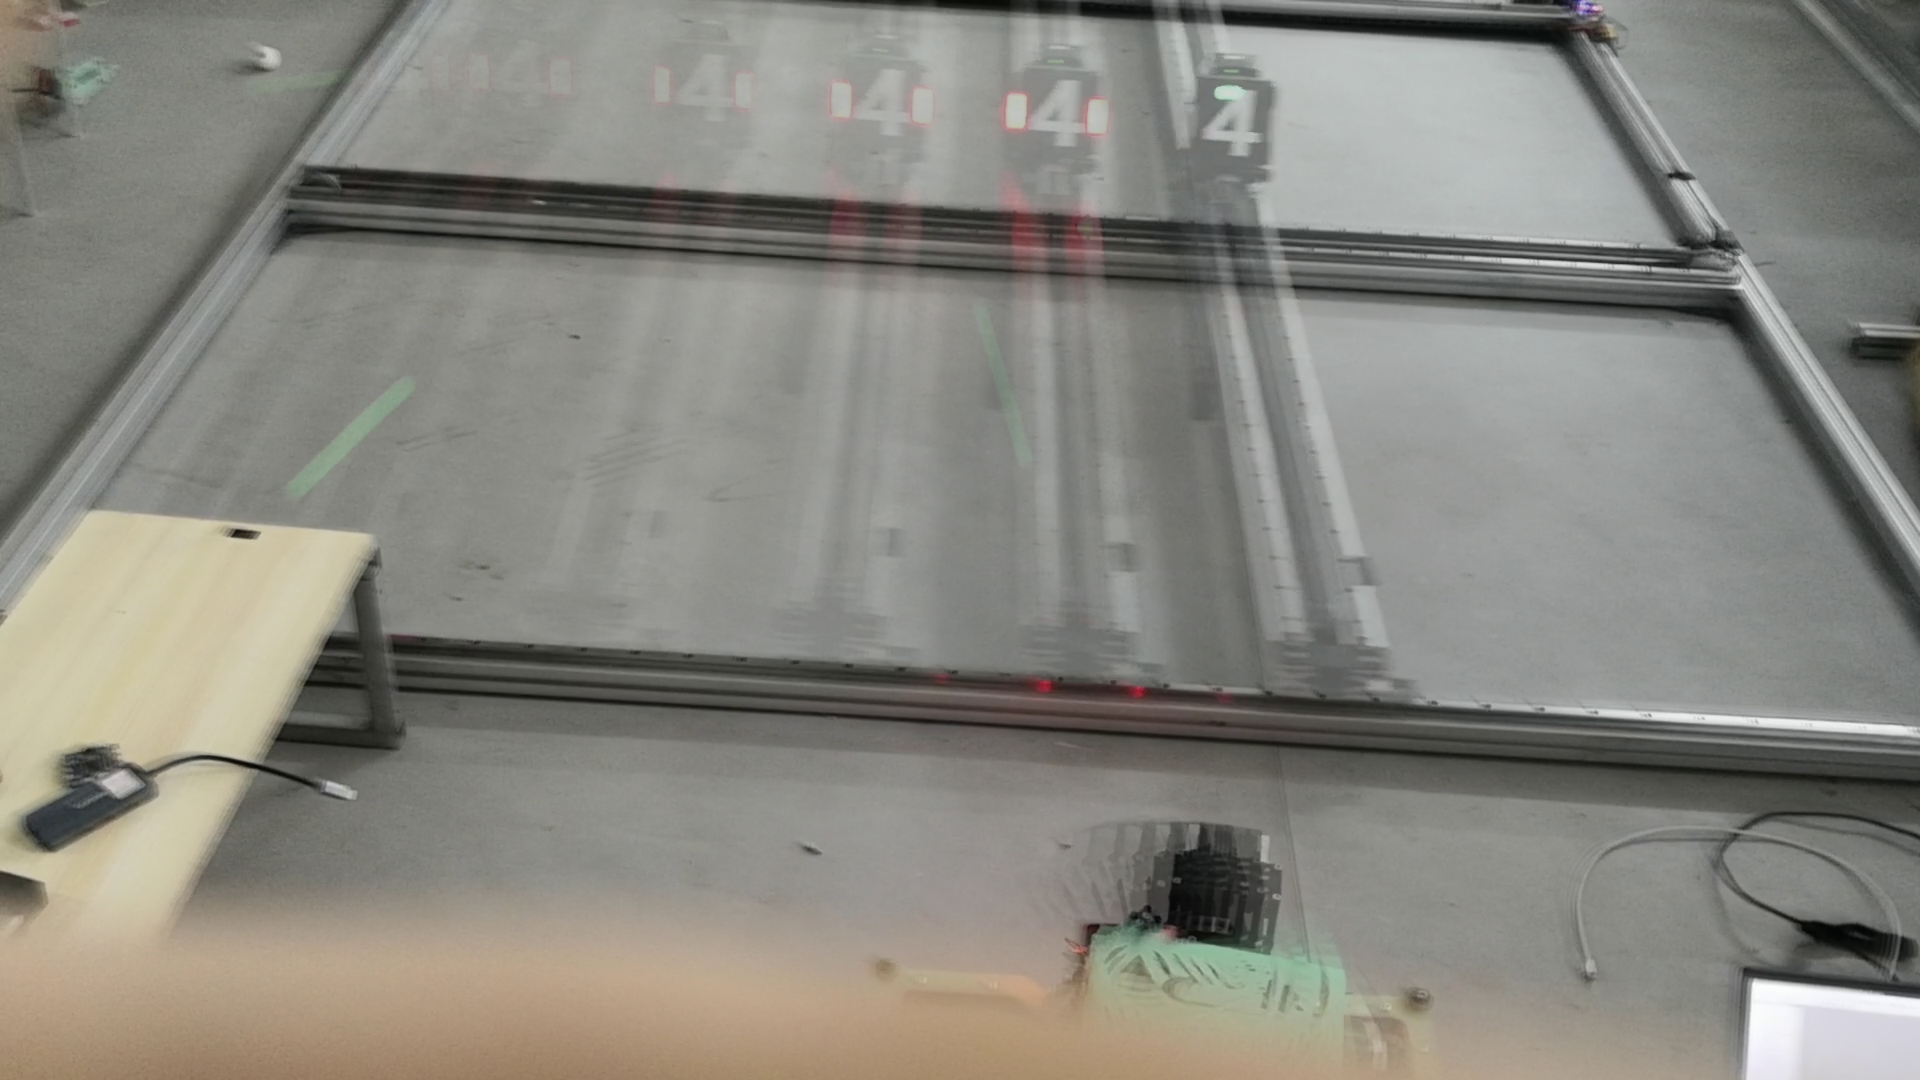
\includegraphics[width=.8\textwidth]{pred_merge.png} 
%     \caption{目标追踪效果展示} 
%     \label{pred_merge} 
% \end{figure} 